% Unofficial University of Cambridge Poster Template
% https://github.com/andiac/gemini-cam
% a fork of https://github.com/anishathalye/gemini
% also refer to https://github.com/k4rtik/uchicago-poster

% !TeX program = lualatex 

\documentclass[final]{beamer}

% ====================
% Packages
% ====================

\usepackage[T1]{fontenc}
\usepackage{lmodern}
\usepackage[size=custom,width=120,height=72,scale=1.0]{beamerposter}
\usetheme{gemini}
\usecolortheme{cam}
\usepackage{graphicx}
\usepackage{booktabs}
\usepackage[numbers]{natbib}
\usepackage{tikz}
\usepackage{pgfplots}
\pgfplotsset{compat=1.14}
\usepackage{anyfontsize}
\usepackage{subcaption}

% ====================
% Lengths
% ====================

% If you have N columns, choose \sepwidth and \colwidth such that
% (N+1)*\sepwidth + N*\colwidth = \paperwidth
\newlength{\sepwidth}
\newlength{\colwidth}
\setlength{\sepwidth}{0.025\paperwidth}
\setlength{\colwidth}{0.3\paperwidth}

\newcommand{\separatorcolumn}{\begin{column}{\sepwidth}\end{column}}

% ====================
% Title
% ====================

\title{Utilizing PID Controller and Kalman Filter for Osoyoo Self-Balancing Robot}

\author{rm -rf humans\inst{1} \and Omar Dsoky \inst{1}}

\institute[shortinst]{\inst{1} Egypt-Japan University of Science and Technology (E-JUST)\\} 

% ====================
% Footer (optional)
% ====================

\footercontent{
  \href{}{} \hfill
         github.com/rm-rf-humans/Osoyoo-Self-Balancing-Robot       \hfill
 \href{}{}}
% (can be left out to remove footer)

% ====================
% Logo (optional)
% ====================

% use this to include logos on the left and/or right side of the header:
% \logoright{\includegraphics[height=7cm]{logo1.pdf}}
% \logoleft{\includegraphics[height=7cm]{logo2.pdf}}

% ====================
% Body
% ====================

\begin{document}

% Refer to https://github.com/k4rtik/uchicago-poster
% logo: https://www.cam.ac.uk/brand-resources/about-the-logo/logo-downloads
\addtobeamertemplate{headline}{}
{
    \begin{tikzpicture}[remember picture,overlay]
      \node [anchor=north west, inner sep=3cm] at ([xshift=0.0cm,yshift=2.5cm]current page.north west)
      {
\includegraphics[height=8.5cm]{logos/ejust.png}}; 

      \node [anchor=north east, inner sep=3cm] at ([xshift=0.0cm,yshift=2.250cm]current page.north east)
      {
\includegraphics[height=7.0cm]{logos/image.png}};
    \end{tikzpicture}
}

\begin{frame}[t]
\begin{columns}[t]
\separatorcolumn

\begin{column}{\colwidth}

  \begin{block}{Mathematical Modeling and Control Design}

   Self-balancing robots are a type of mobile robot that can maintain an upright position while moving in which applies inverse pendulum control due to its nonlinearity and unstable nature dynamic system. The pendulum will simply fall over the cart is not moved to balance it. The mathematical model obtained is in the form of non-linear equations that describe the motion of the inverted pendulum: 
   $$
   	(M + m)\ddot{x} + f\dot{x} + m\ddot{\theta}lcos(\theta) - ml\dot{\theta}^2sin(\theta) = F 
   $$
   $$
   	(I + ml^2)\ddot{\theta} + mglsin(\theta) - ml\ddot{x}cos(\theta) = 0
   $$
   The system can be linearized around the equilibrium point, which is the upright position of the pendulum, by approximating $sin(\theta) = \theta$ assuming $\theta$ is small and substituting $cos(\theta) = 1$ \cite{Abdelgawad2024-wr}. The linearized equations can be represented in state-space form as follows:
   $$
   	(I + ml^2)\ddot{\theta} + mgl\theta - ml\ddot{x} = 0
   $$
   $$
   	(M + m)\ddot{x} + f\dot{x} - m\ddot{\theta}l = u
   $$
   The state-space representation of the system can be obtained by defining the state vector as $x = [x, \dot{x}, \theta, \dot{\theta}]^T$ and the input vector as $u = [F]^T$. Moreover, the system can be in close loop control by using a PID controller to adjust the input force $F$ based on the error between the desired angle and the actual angle. However, the PID controller alone may not be sufficient to achieve the desired performance. Therefore, Kalman and Complementary filters can be used to estimate the state of the system based on noisy measurements of the angle and angular velocity. 
   %  \begin{figure}
   %   \centering
    %  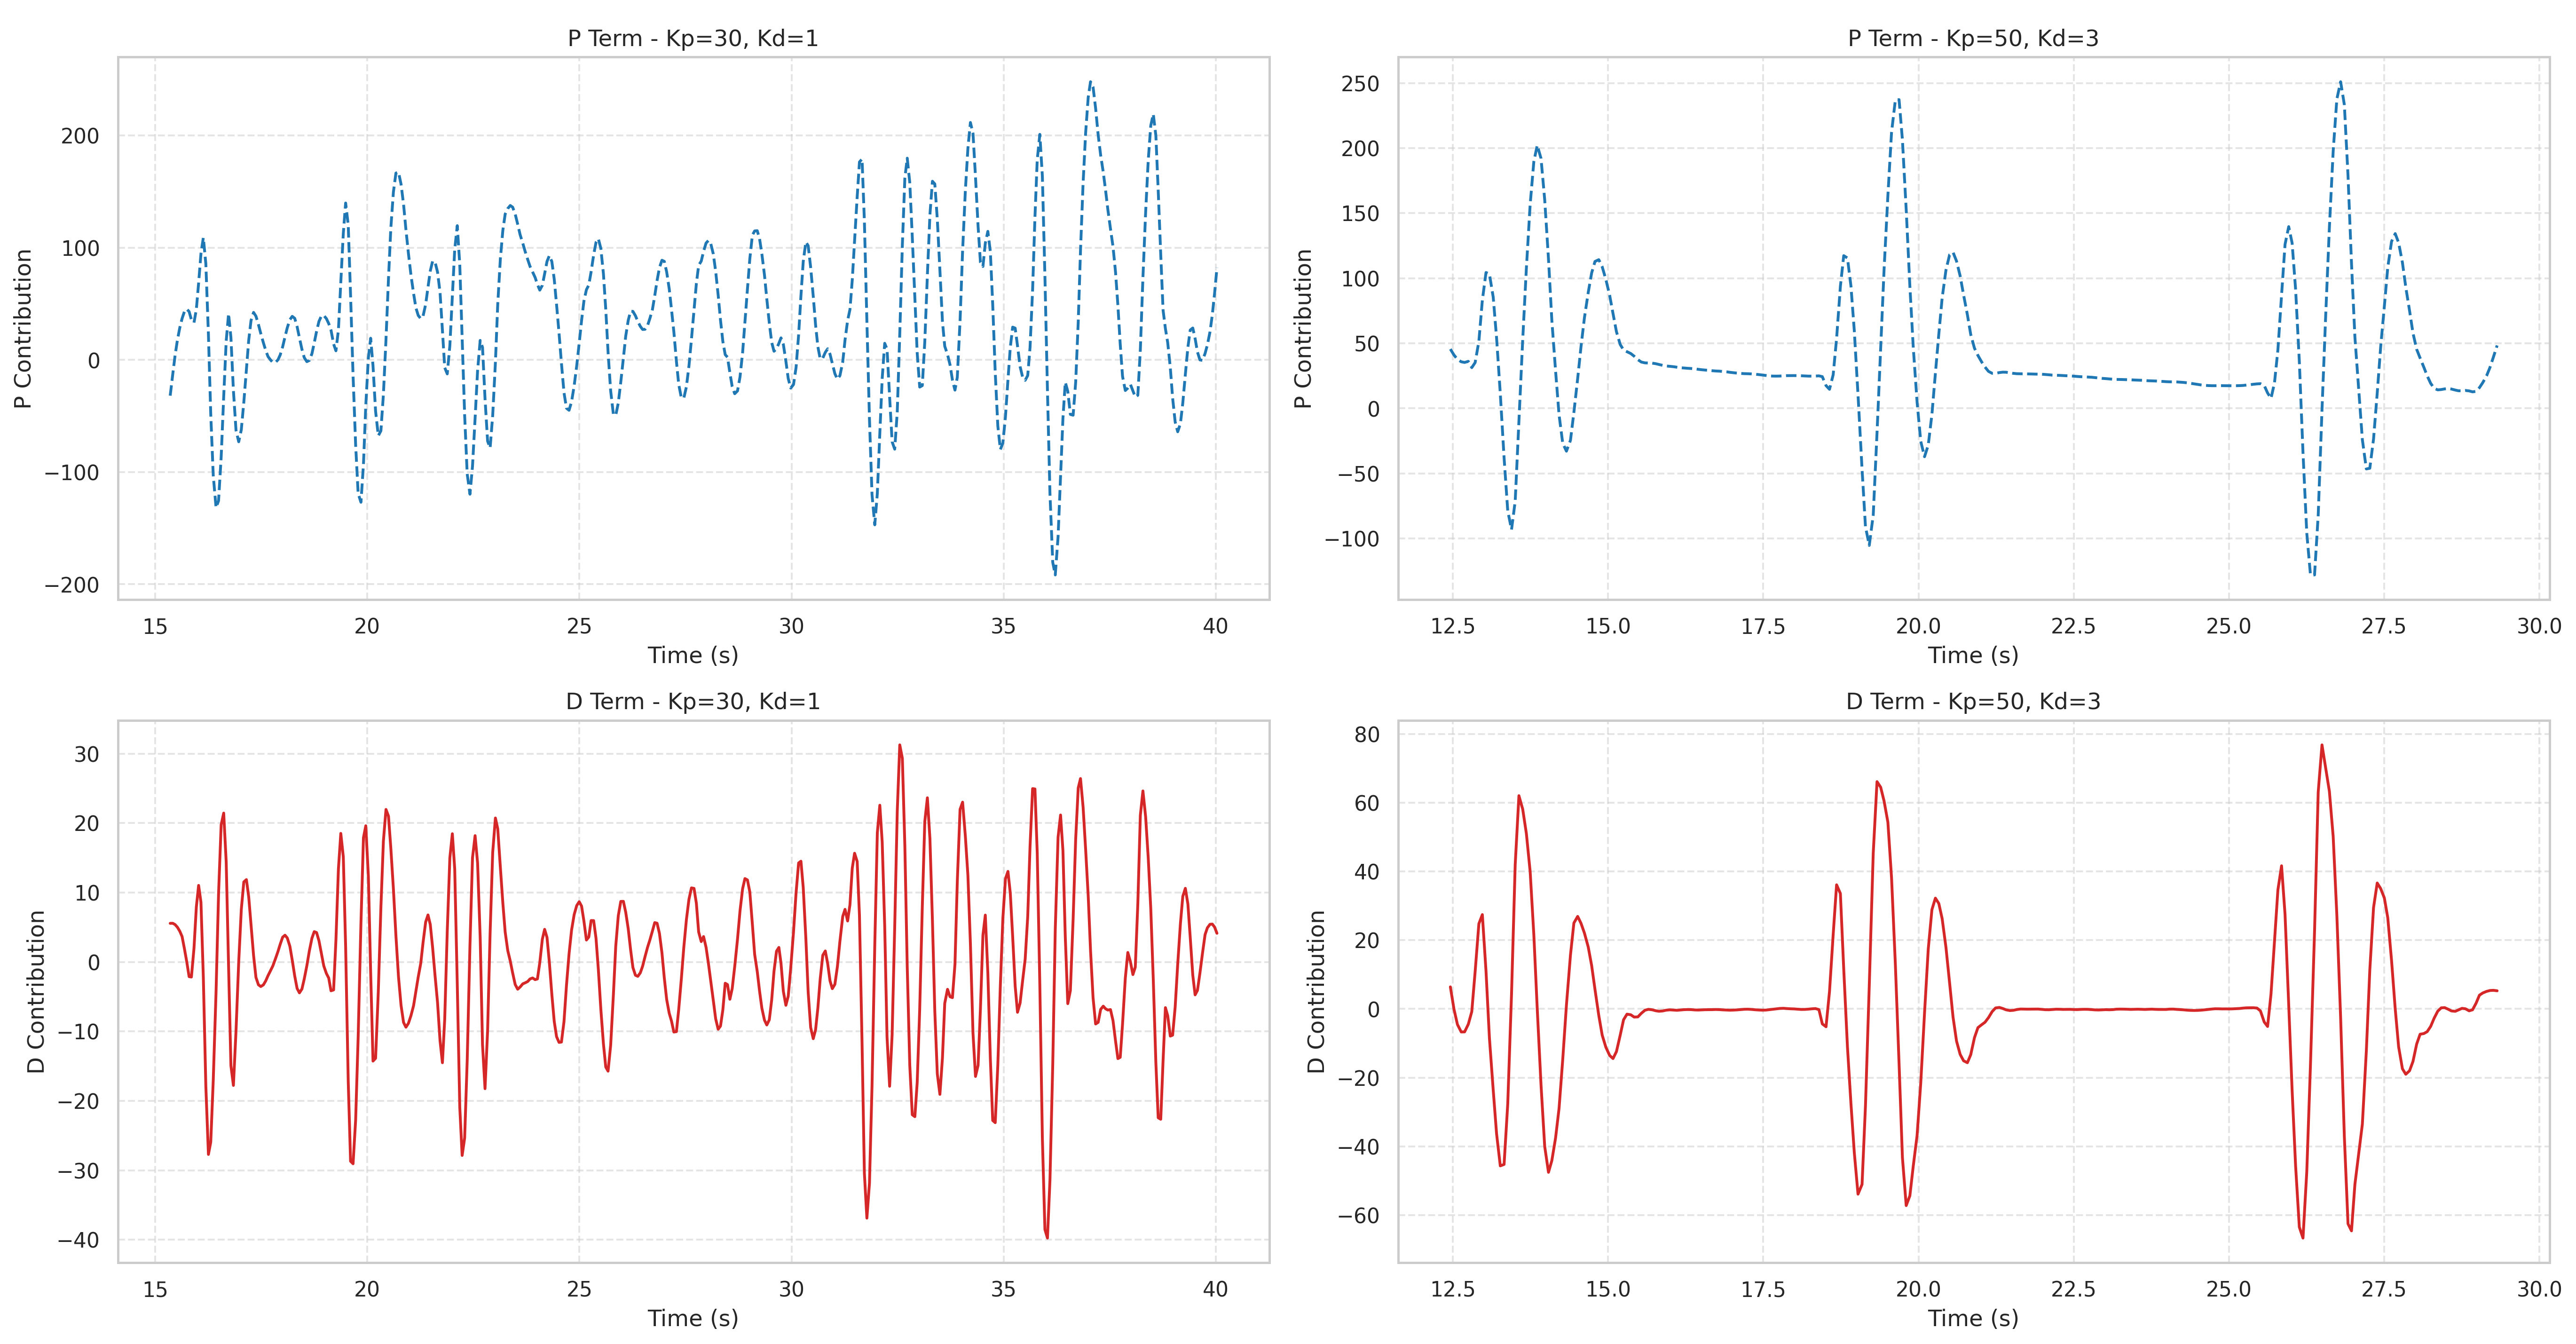
\includegraphics[width=1.0\textwidth]{logos/pid_pd_matrix_comparison_.png}      
     % \caption{A figure caption.}
    %\end{figure}
  \end{block}


  \vspace{0.8em}


  \begin{alertblock}{Sensor Fusion and Filtering}


	  To obtain a reliable estimate of the pitch angle \( \theta \), measurements from both sensors must be fused. The accelerometer provides an absolute but noisy estimate relative to gravity, and the gyroscope provides the angular velocity \( \dot{\theta}_{\text{gyro}} \):
\[
\theta_{\text{acc}} = \text{atan2}(a_y, a_z)
\]
\[
\theta_{\text{gyro}} = \dot{\theta}_{\text{gyro}} \cdot dt + \theta_{\text{prev}}
\]
However, due to integration drift, gyroscope readings are unreliable over time. Sensor fusion techniques are therefore necessary to obtain a more stable and accurate angle estimate.
The complementary filter fuses gyroscope and accelerometer data using a weighted average:
\[
\theta_{\text{filter}} = \alpha \cdot \theta_{\text{gyro}} + (1 - \alpha) \cdot \theta_{\text{acc}}
\]
A more advanced alternative is the Kalman filter, which estimates the true state of a system by minimizing the error covariance through a recursive prediction-correction loop:
\[
P_{k|k-1} = P_{k-1|k-1} + Q
\]
The Kalman gain is then computed:
\[
K_k = \frac{P_{k|k-1}}{P_{k|k-1} + R}
\]
Next, the predicted angle is corrected based on the accelerometer measurement:
\[
\hat{\theta}_{k|k} = \hat{\theta}_{k|k-1} + K_k \cdot (\theta_{\text{acc}} - \hat{\theta}_{k|k-1})
\]
\[
P_{k|k} = (1 - K_k) \cdot P_{k|k-1}
\]
Compared to the complementary filter, the Kalman filter provides more accurate results at the cost of higher computational complexity and the need for precise tuning of the process noise \( Q \) and measurement noise \( R \).

\end{alertblock}

\end{column}

\separatorcolumn

\begin{column}{\colwidth}

\begin{block}{System Response with PID Control and Gyroscope}	
\begin{figure}[h!]
    \centering
    \begin{subfigure}[t]{0.48\textwidth}
        \centering
        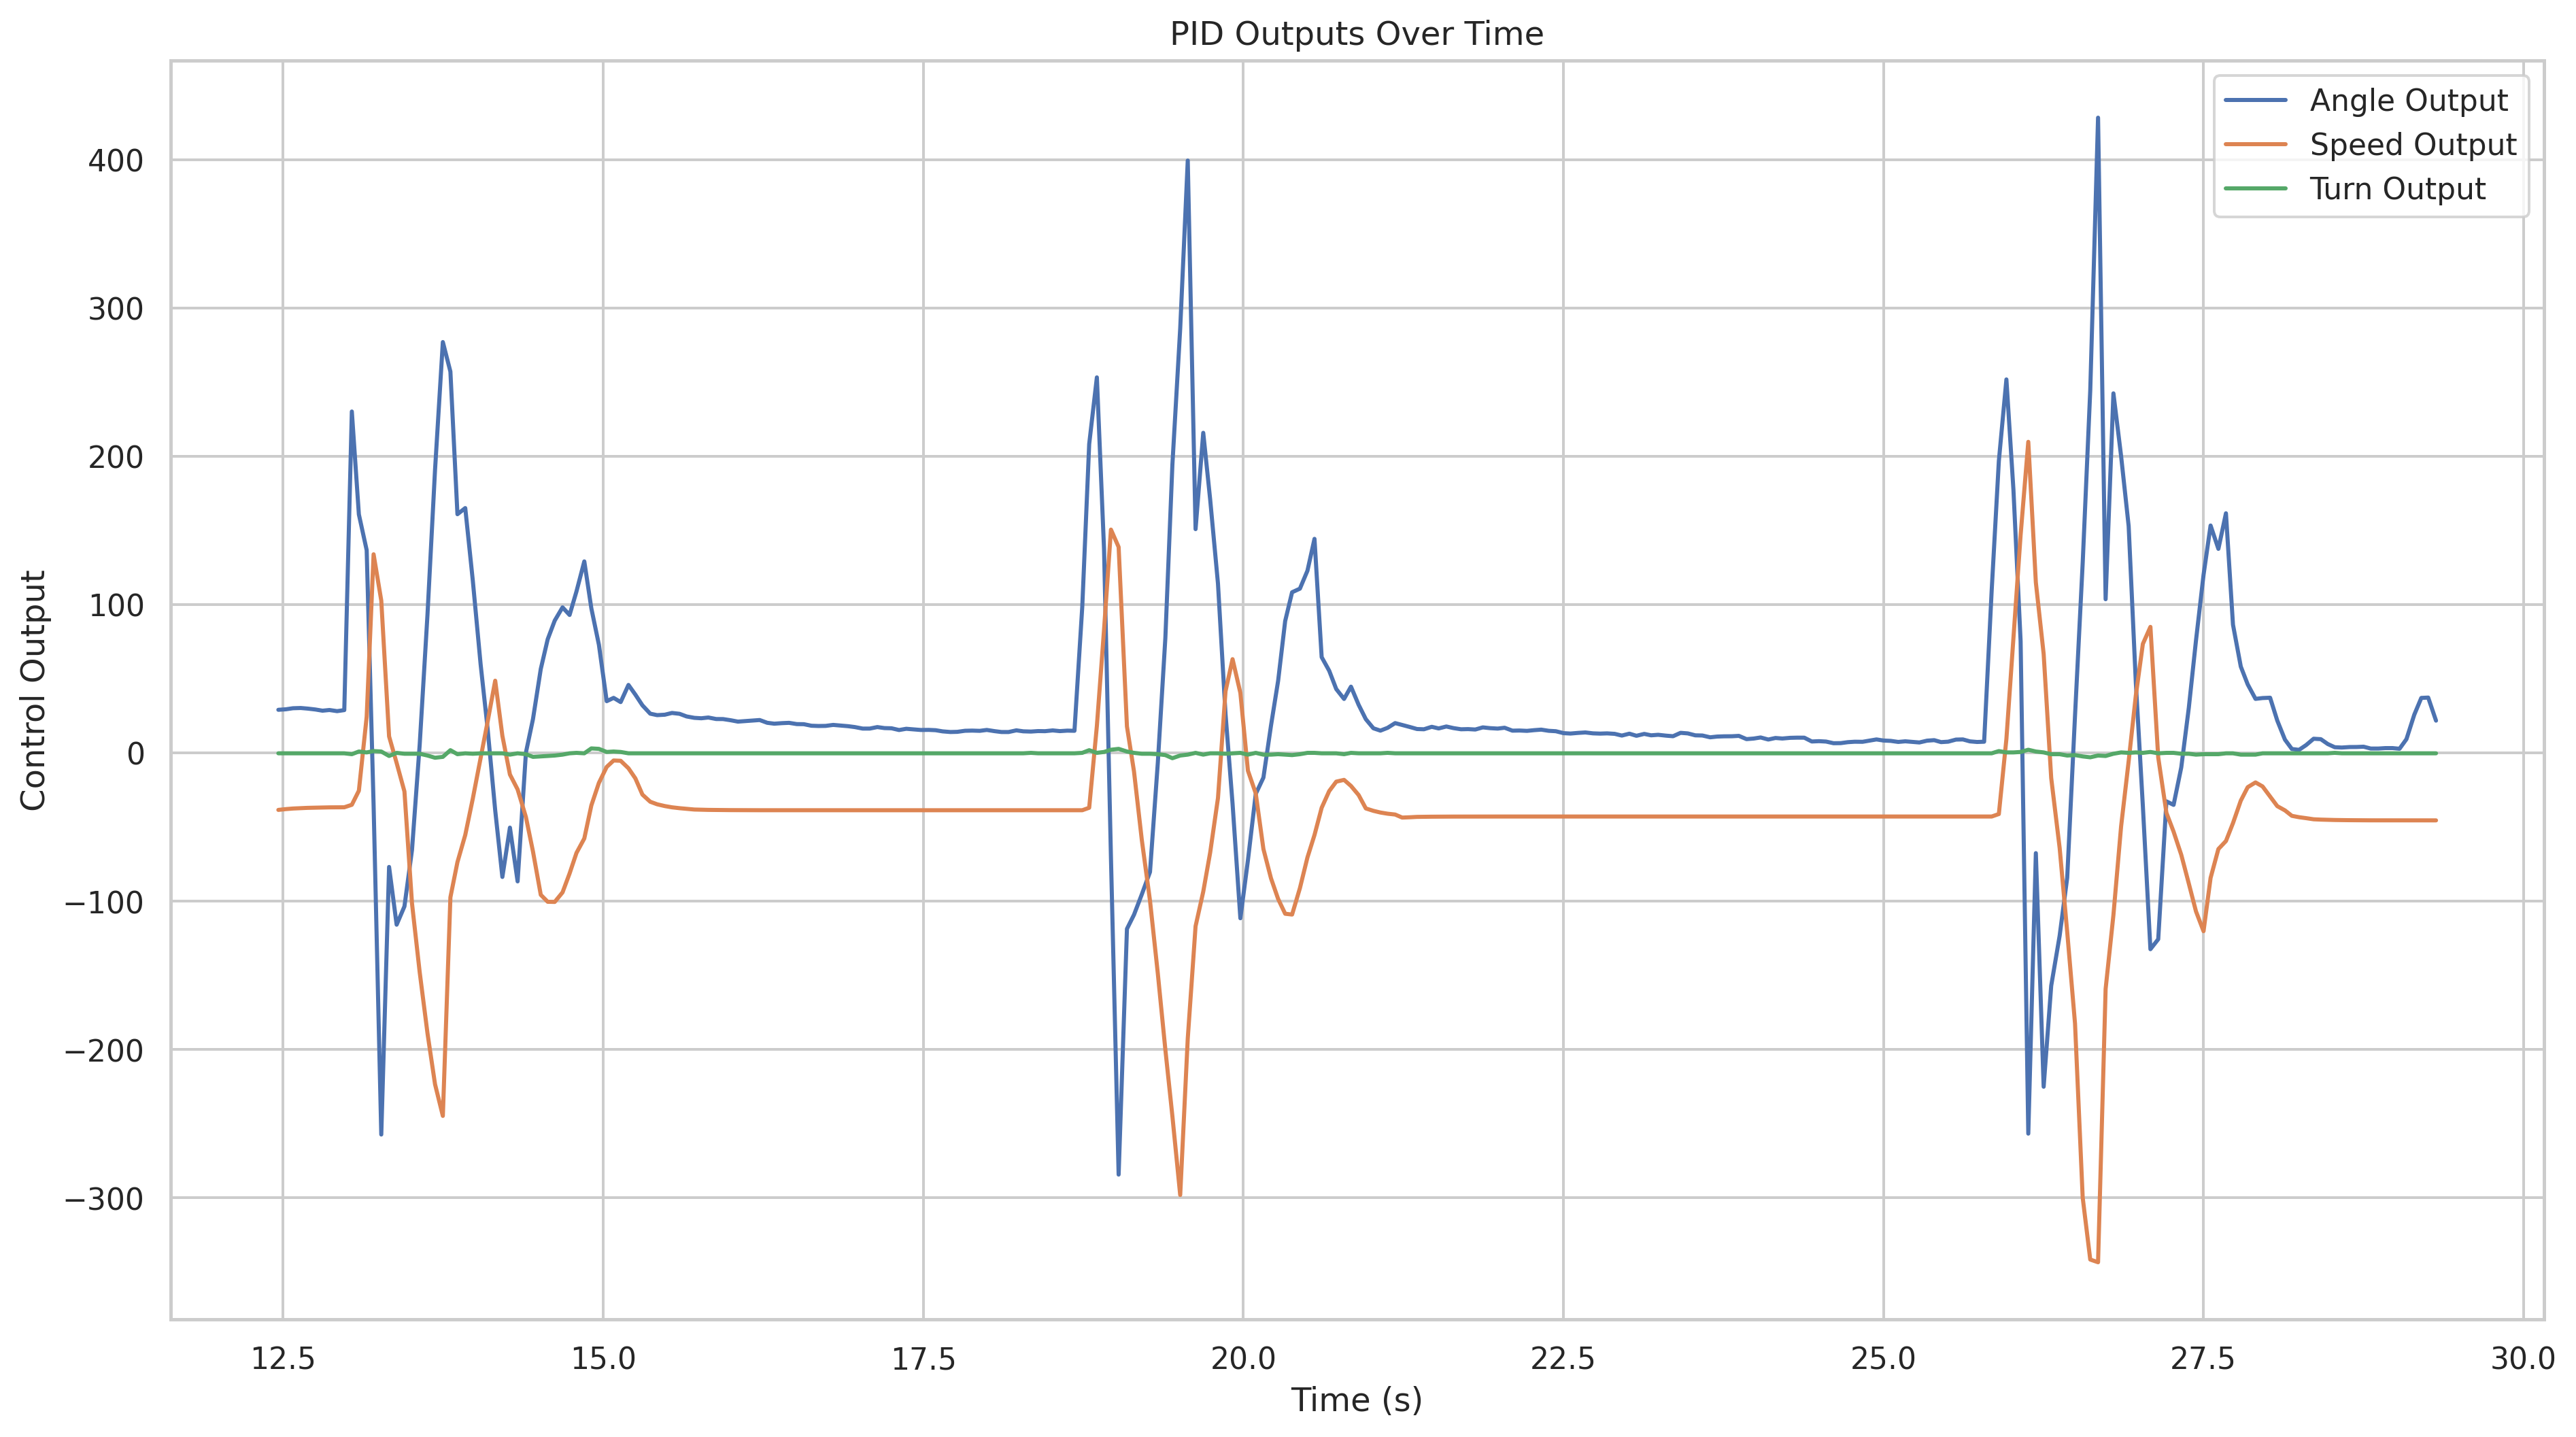
\includegraphics[width=\linewidth]{logos/pid_outputs_.png}
        \caption{Outputs from PID control}
        \label{fig:comp_filter}
    \end{subfigure}
    \hfill
    \begin{subfigure}[t]{0.48\textwidth}
        \centering
        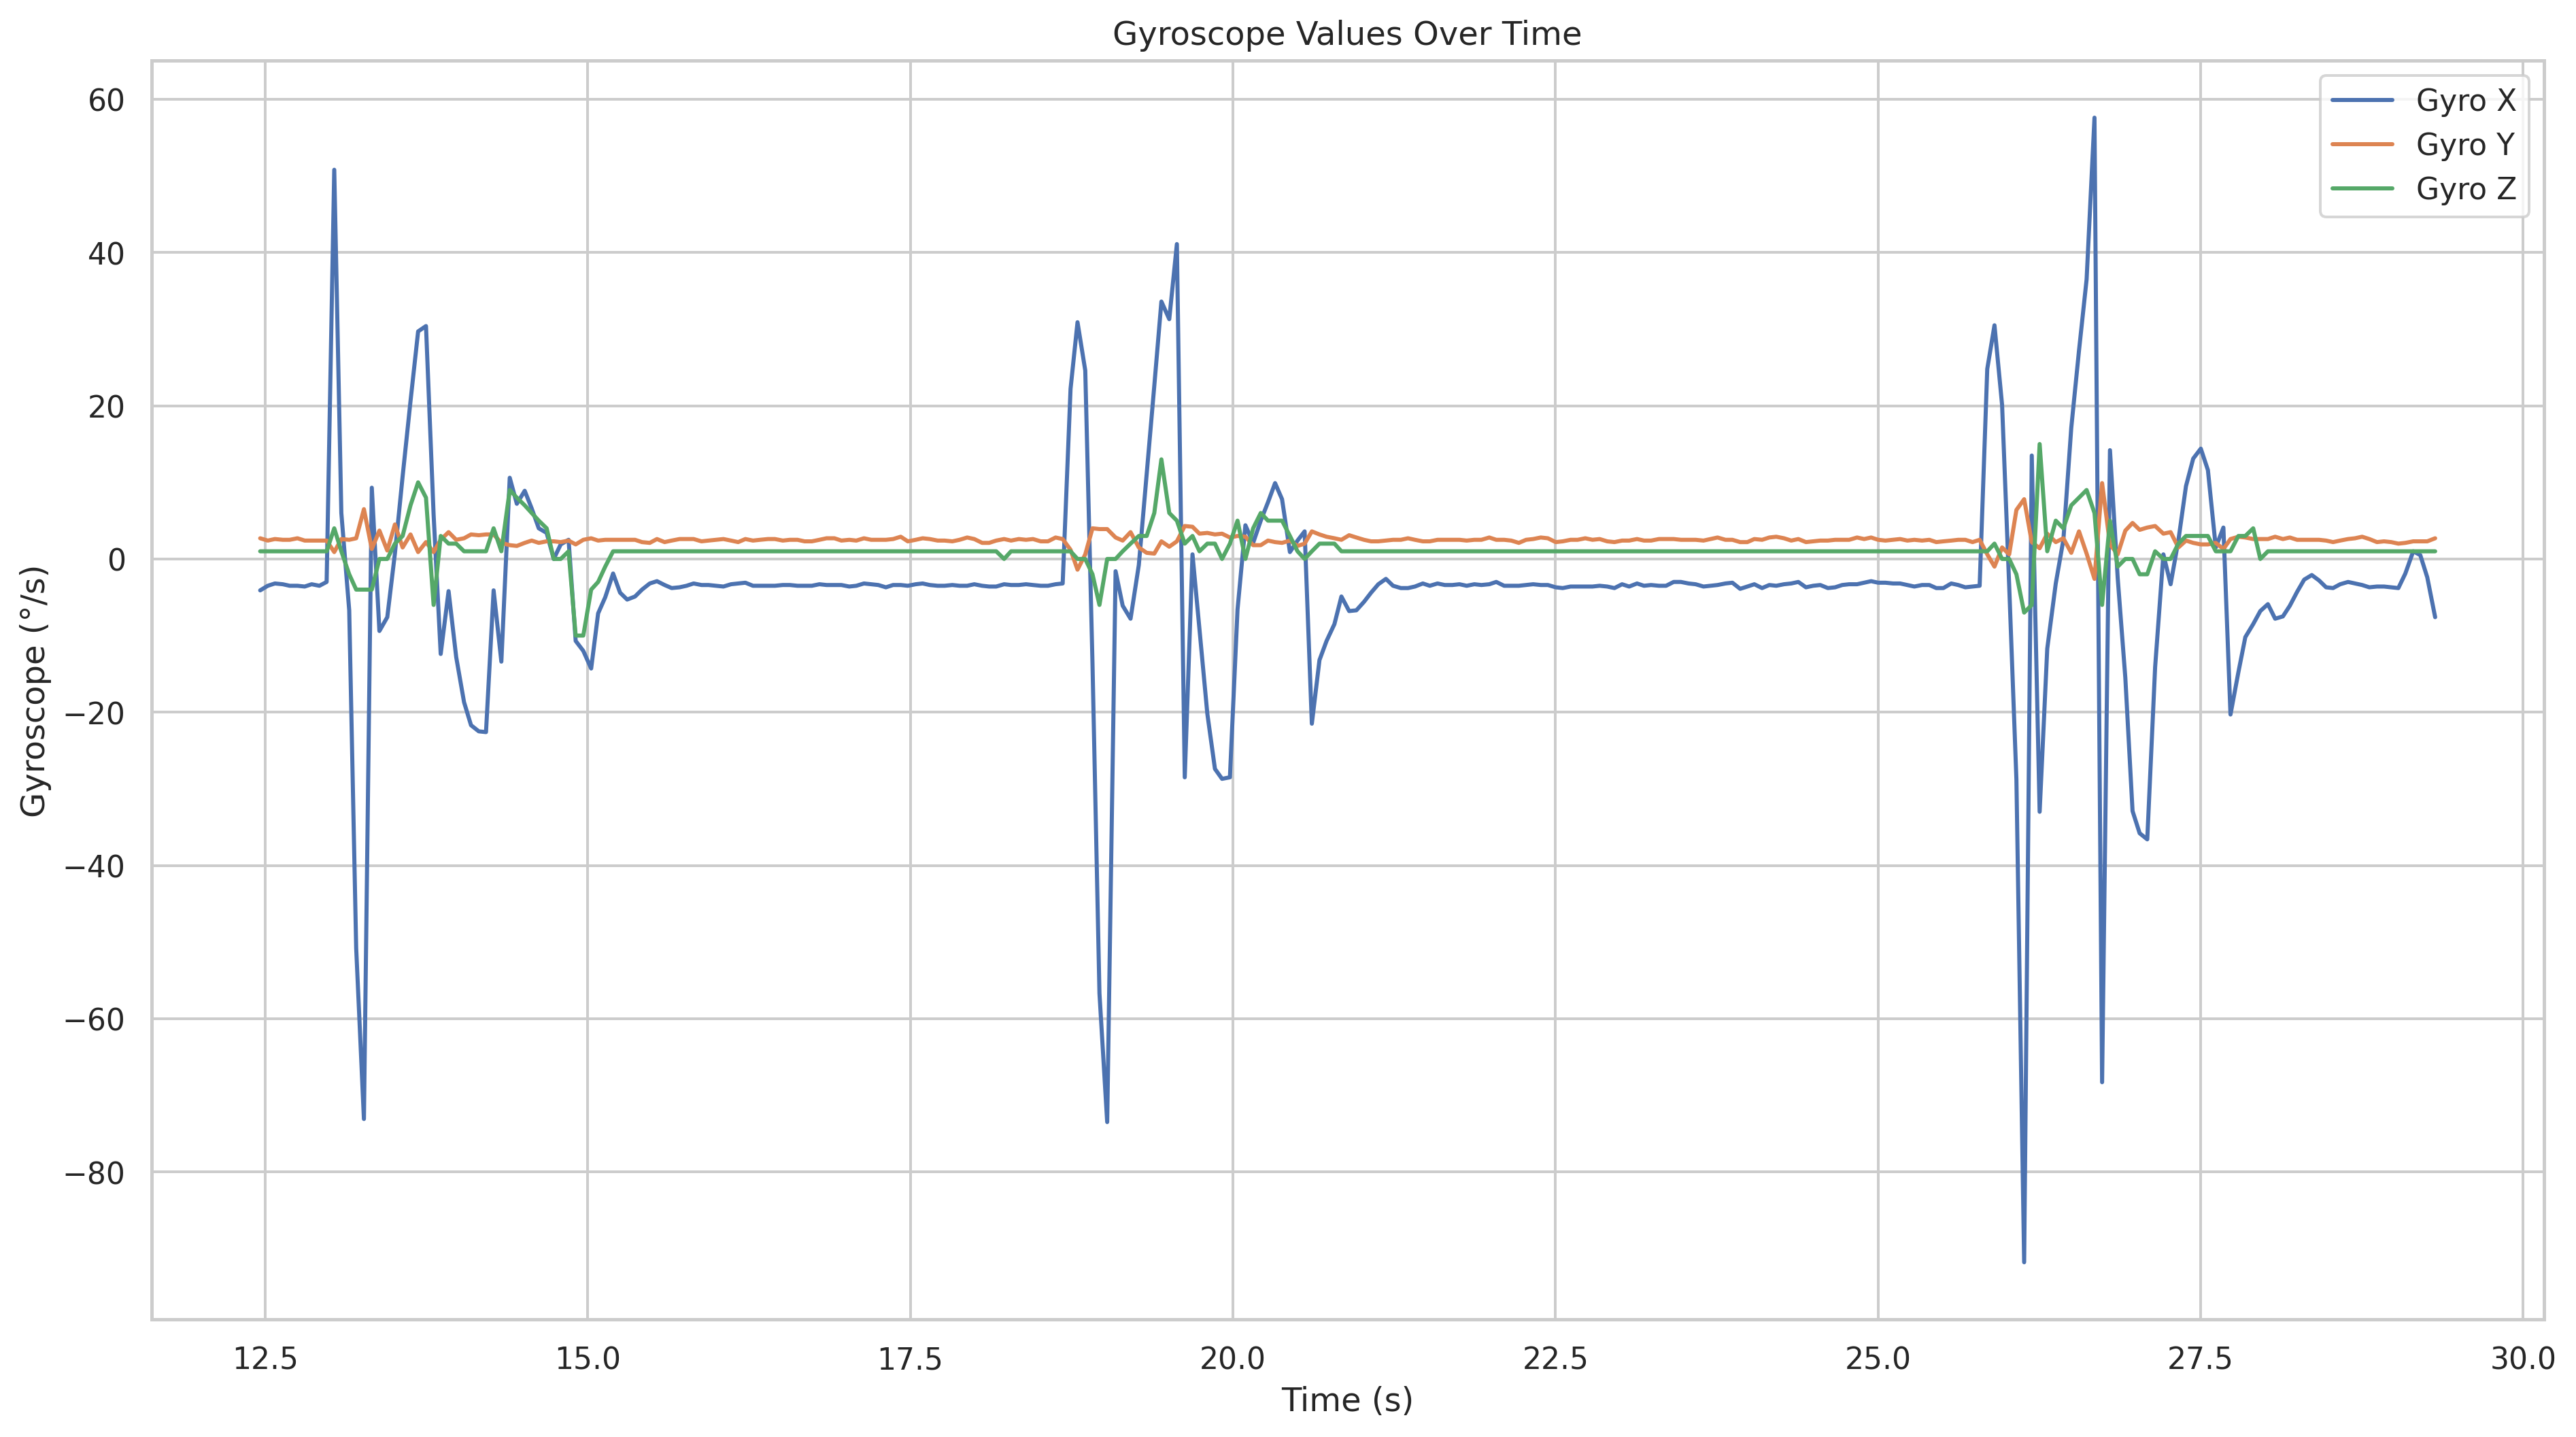
\includegraphics[width=\linewidth]{logos/gyro_values_.png}
        \caption{Readings from the filtered gyroscope}
        \label{fig:kalman_filter}
    \end{subfigure}
    \caption{System response showing PID controller outputs and filtered gyroscope readings during robot balancing.}
    \label{fig:filters}
\end{figure}
  \end{block}
  \begin{block}{Kinematics and Mechanical Design Using CAD}

	The intricate process of mathematical modeling pertaining to the robotic system combined with the sophisticated design approach utilizing CAD methodologies for the same robotic entity.
   \vspace{1em}

\begin{columns}
\begin{column}{0.5\textwidth}
\begin{center}
      \begin{figure}
	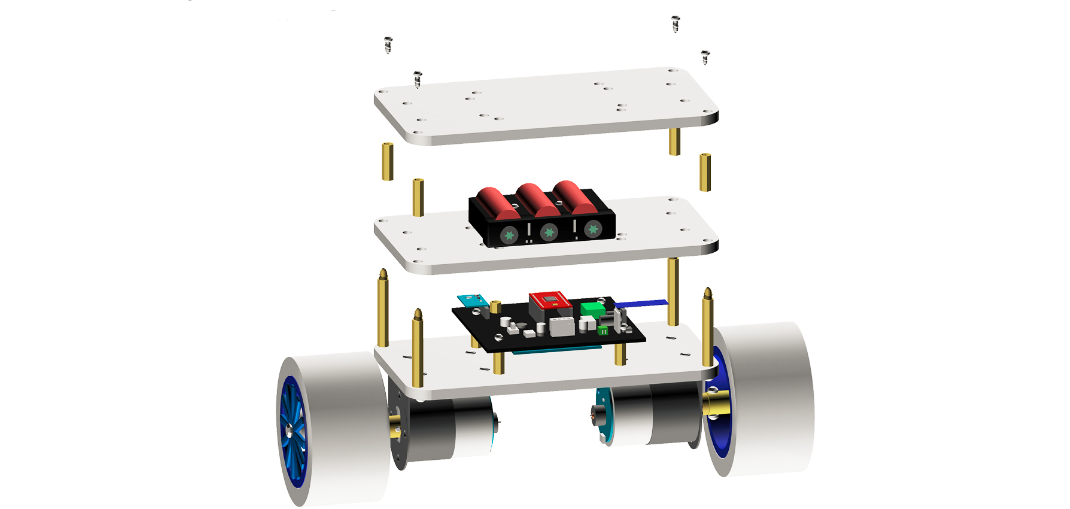
\includegraphics[width=1.0\textwidth]{logos/CAD.png}
      \caption{CAD design of the Osoyoo self-balancing robot.}
    \end{figure}
   \end{center}
\end{column}
\begin{column}{0.5\textwidth}  %%<--- here
   \begin{center}
      \begin{figure}
	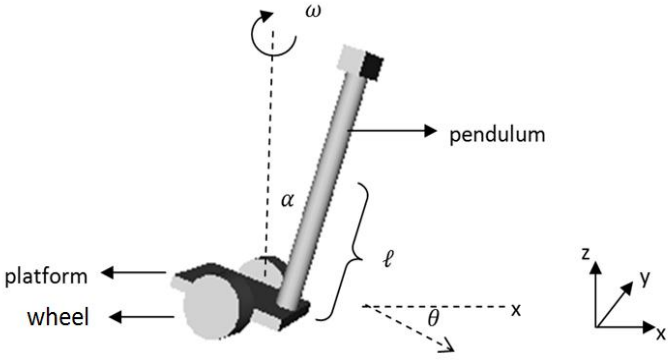
\includegraphics[width=.880\textwidth]{logos/Kin.png}
	\caption{A Modeling and Kinematics of the robot [2].}
    \end{figure}
   \end{center}
\end{column}
\end{columns}


  \end{block}

  \begin{block}{System Performance and Results}
	  \begin{figure}
		\centering
		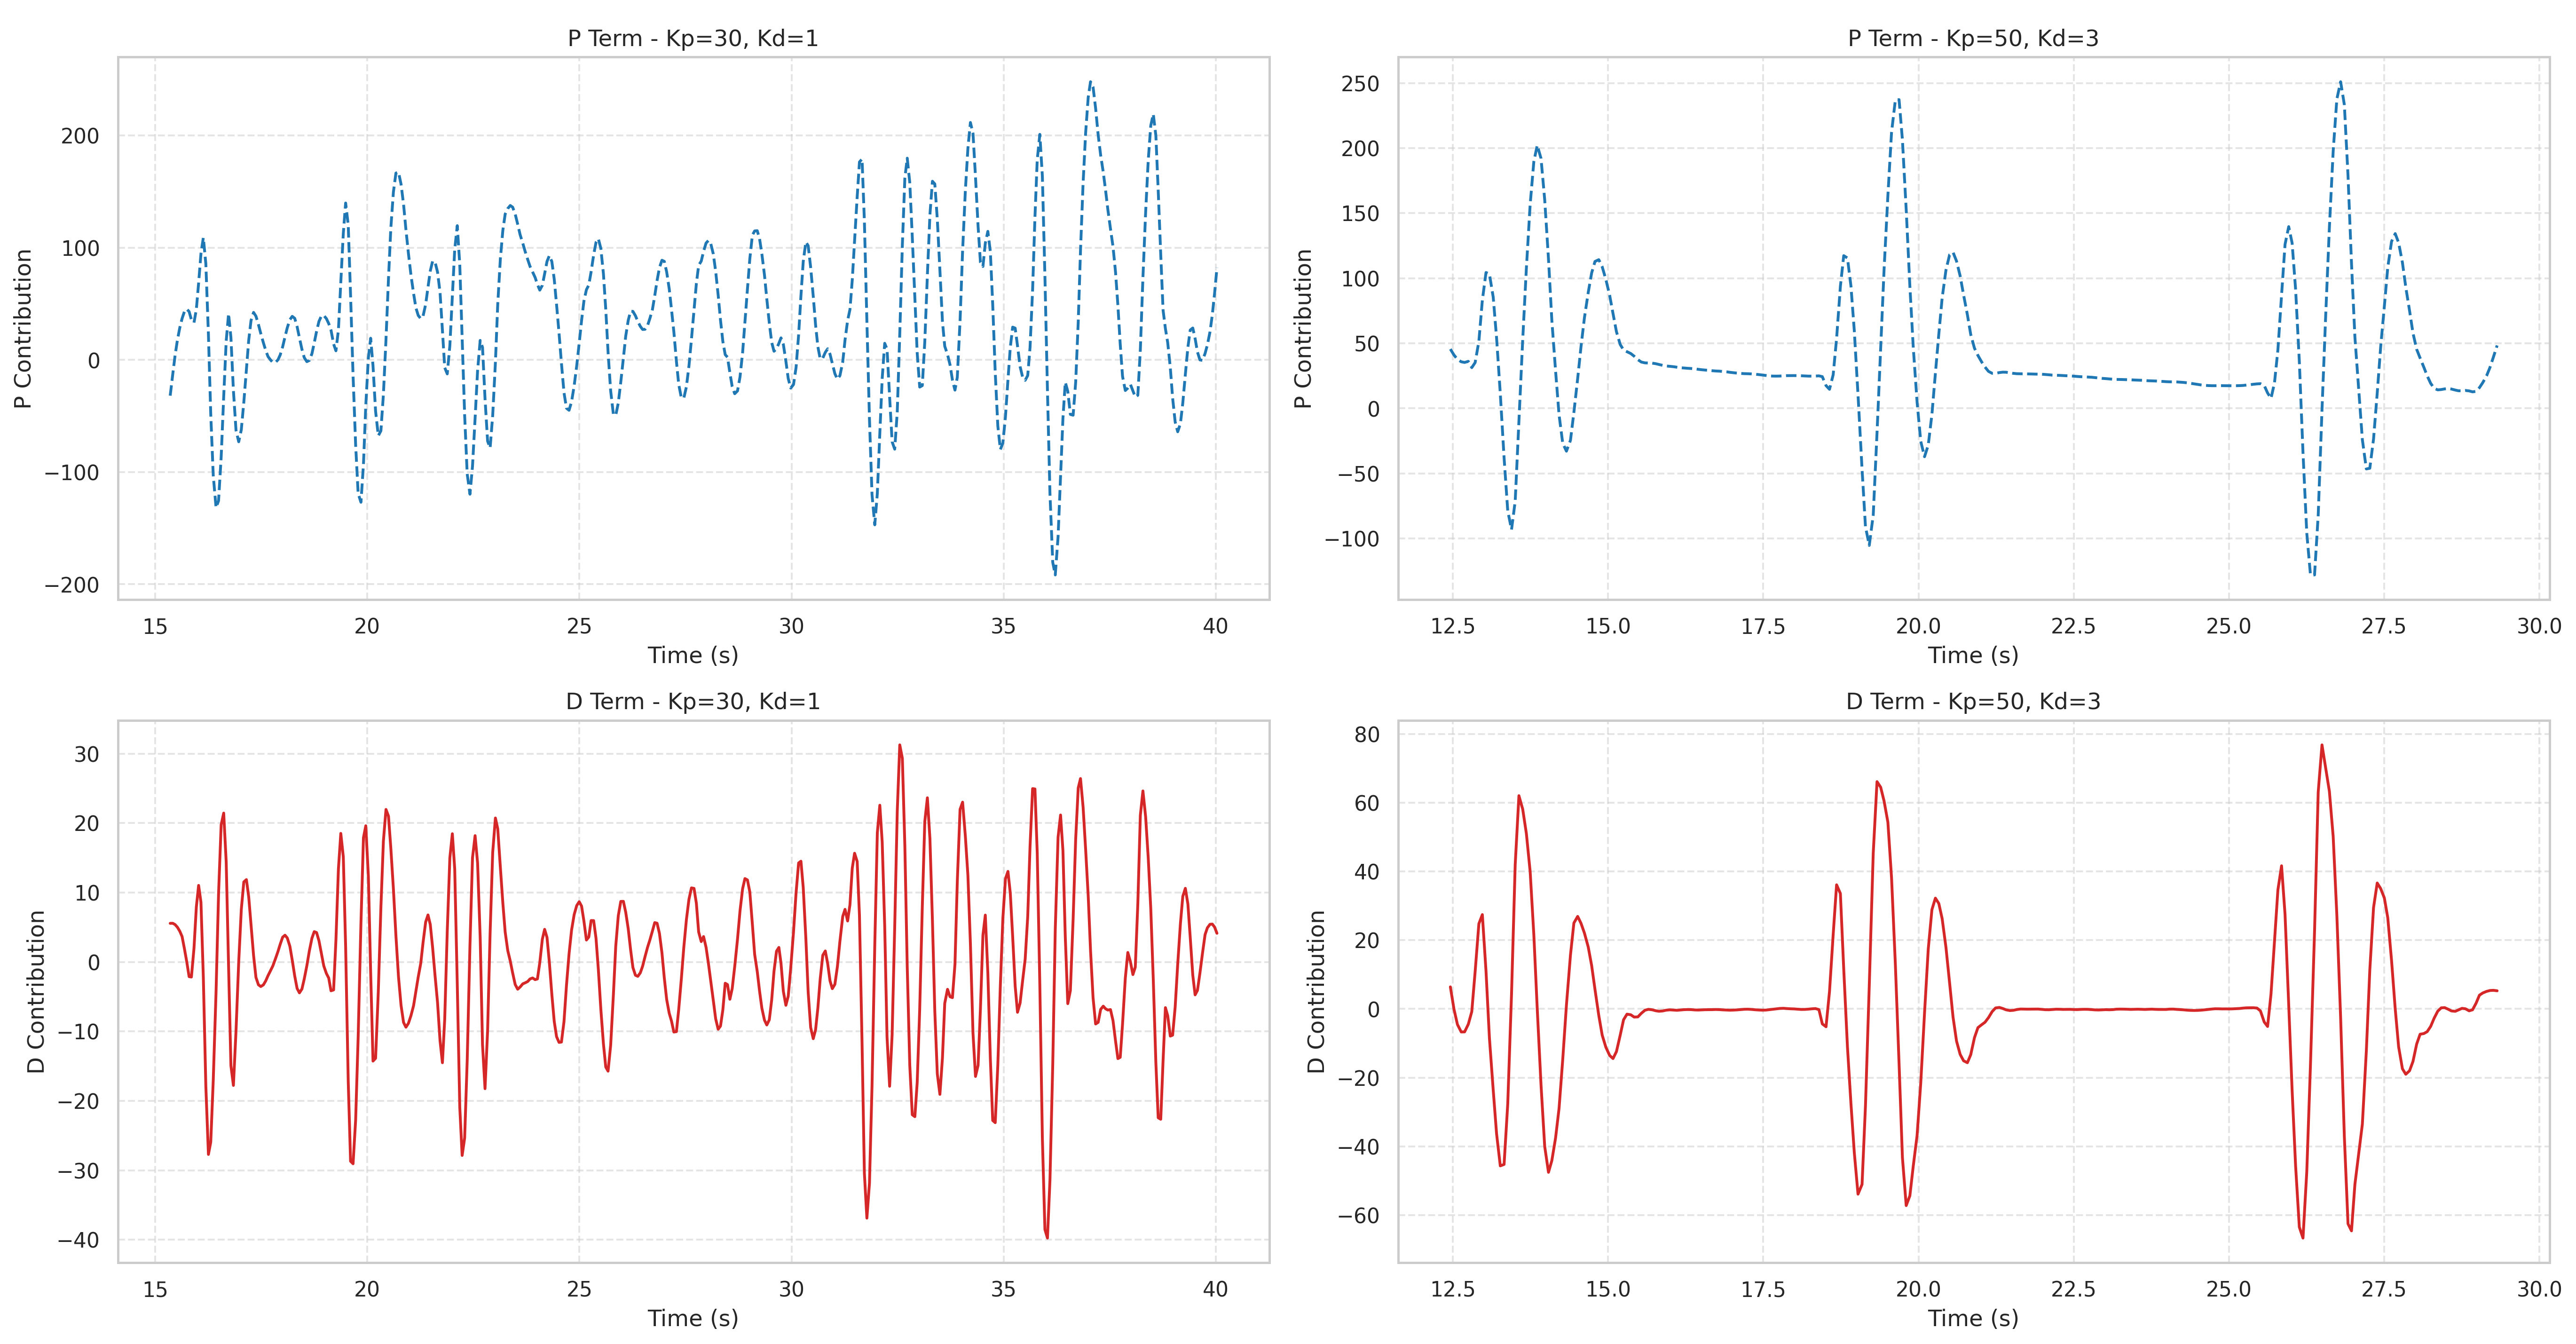
\includegraphics[width=01.0\textwidth]{logos/pid_pd_matrix_comparison_.png}
		\caption{Simulated response and validation of PID controller through comparison with PD controller.}
	  \end{figure}
  \end{block}

\end{column}

\separatorcolumn

\begin{column}{\colwidth}

  \begin{exampleblock}{PID Controller Fundamentals and Transfer Function}

	  The PID (Proportional-Integral-Derivative) controller is a fundamental feedback mechanism widely used in control systems. It calculates the control signal \( u(t) \) based on the error \( e(t) \), which is the difference between the desired setpoint and the current system output [3].

\[
u(t) = K_p e(t) + K_i \int e(t)\,dt + K_d \frac{de(t)}{dt}
\]

Where \( K_p \): Proportional gain – reacts to the current error, \( K_i \): Integral gain – accumulates past errors, \& \( K_d \): Derivative gain – predicts future error based on the rate of change.

\heading{PID Transfer Function:}

Applying the Laplace transform to the time-domain PID expression yields:
\[
U(s) = \left(K_p + \frac{K_i}{s} + K_d s\right) E(s)
\]
\heading{Complete Closed-Loop View:}

The system operates in a feedback loop:
\[
r(t) \xrightarrow{-} e(t) = r(t) - \hat{x}(t) \xrightarrow{G_{\text{PID}}} u(t) \xrightarrow{Plant} y(t) \xrightarrow{Sensors} z(t) \xrightarrow{\text{Kalman Filter}} \hat{x}(t)
\]
The PID controller improves system stability, responsiveness, and accuracy by combining these three components.
 
\end{exampleblock}


  \begin{block}{Gyroscope Noise Filtering Results}
Gyroscopes are essential components in inertial measurement units (IMUs) for estimating angular velocity. However, raw gyroscope data is often affected by high-frequency noise, which can degrade the quality of orientation estimation over time. 

Table~\ref{tab:gyro_noise} shows the effectiveness of the applied filtering method on each of the gyroscope axes. The percentage values represent the reduction in noise power compared to the unfiltered signal. Results indicate significant noise attenuation across all three axes, with 99\% noise reduction.
\begin{table}[h!]
  \centering
  \renewcommand{\arraystretch}{1.3}
  \caption{Noise reduction percentages for gyroscope axes after filtering.}
  \label{tab:gyro_noise}
  \begin{tabular}{c@{\hspace{2cm}}c}
    \toprule
    \textbf{Gyroscope Axis} & \textbf{Noise Reduction} \\
    \midrule
    X & 99.24\% \\
    Y & 99.23\% \\
    Z & 99.52\% \\
    \bottomrule
  \end{tabular}
\end{table}

These  results demonstrate the reliability of sensor fusion algorithms in mitigating noise, ultimately leading to more stable and accurate orientation estimates in real-time applications. 
 \end{block}

  \begin{block}{References}

    \nocite{*}
    \footnotesize{\bibliographystyle{plainnat}\bibliography{poster}}

  \end{block}

\end{column}

\separatorcolumn%
\end{columns}
\end{frame}

\end{document}
